
% part 4
\section{Twisted поэзия\label{sec:part4}}

\subsection{Наш первый Twisted клиент}

Twisted используется в основном для написания серверов. 
Конечно, можно его использовать для написать клиентов, 
что существенно проще, чем написание серверов. Мы начнем с 
простого: с написания клиента. 
Давайте попробуем наш первый поэтический клиент, 
написанный с использованием Twisted. Исходный код  
можно найти в 
\href{http://github.com/jdavisp3/twisted-intro/blob/master/twisted-client-1/get-poetry.py}{twisted-client-1/get-poetry.py}. Сначала нужно запустить поэтические сервера:

\begin{scriptsize}\begin{verbatim}
python blocking-server/slowpoetry.py --port 10000 poetry/ecstasy.txt --num-bytes 30
python blocking-server/slowpoetry.py --port 10001 poetry/fascination.txt
python blocking-server/slowpoetry.py --port 10002 poetry/science.txt
\end{verbatim}\end{scriptsize}

Затем запустите клиент следующим образом:

\begin{scriptsize}\begin{verbatim}
python twisted-client-1/get-poetry.py 10000 10001 10002
\end{verbatim}\end{scriptsize}

И получится следующий вывод:

\begin{scriptsize}\begin{verbatim}
Task 1: got 60 bytes of poetry from 127.0.0.1:10000
Task 2: got 10 bytes of poetry from 127.0.0.1:10001
Task 3: got 10 bytes of poetry from 127.0.0.1:10002
Task 1: got 30 bytes of poetry from 127.0.0.1:10000
Task 3: got 10 bytes of poetry from 127.0.0.1:10002
Task 2: got 10 bytes of poetry from 127.0.0.1:10001
...
Task 1: 3003 bytes of poetry
Task 2: 623 bytes of poetry
Task 3: 653 bytes of poetry
Got 3 poems in 0:00:10.134220
\end{verbatim}\end{scriptsize}

Также как мы это делали для нашего асинхронного клиента, 
не использующего Twisted. И это неудивительно, что клиент 
выполняет тоже, что и раньше. Давайте посмотрим на исходный код 
для того, чтобы понять как он работает. Откройте их в редакторе, чтобы можно было 
смотреть на то, что мы будем обсуждать.


Заметьте, что как было упомянуто, мы начнем изучать Twisted с 
очень низкоуровневых API. Проходя по абстракциям Twisted снизу 
вверх, мы сможем изучить Twisted изнутри и сверху. Это означает, что 
мы изучим многие API, которые обычно не используются при 
написании реального кода. Запомните, что первоначальные примеры - это не 
то, как надо писать боевой код, а лишь способ изучения Twisted.


Twisted клиент начинается с создания множества объектов типа 
\href{http://github.com/jdavisp3/twisted-intro/blob/master/twisted-client-1/get-poetry.py#L53}{PoetrySocket}. 
PoetrySocket инициализирует себя сам созданием сетевого 
сокета, соединенного с сервером и выставленного в неблокирующий режим: 

\begin{scriptsize}\begin{verbatim}
self.sock = socket.socket(socket.AF_INET, socket.SOCK_STREAM)
self.sock.connect(address)
self.sock.setblocking(0)
\end{verbatim}\end{scriptsize}


Конечно, в дальнейшем мы будет иметь дело с 
абстрациями, при использовании которых не надо 
работать с сокетами, но сейчас нам нужно работать с ними. 
После создания сетевого соединения, PoetrySocket подставляет 
себя в reactor через метод addReader:

\begin{scriptsize}\begin{verbatim}
# tell the Twisted reactor to monitor this socket for reading
from twisted.internet import reactor
reactor.addReader(self)
\end{verbatim}\end{scriptsize}

Этот метод дает Twisted файловый дескриптор, который он должен 
проверить на предмет приходящих данных. Почему мы передаем 
Twisted объект вместо файлового дескриптора и callback'а? 
И как Twisted узнает, что делать с этим объектом, ведь  
Twisted не содержит кода, относящегося к поэзии? Откройте 
\href{http://twistedmatrix.com/trac/browser/tags/releases/twisted-8.2.0/twisted/internet/interfaces.py}{twisted.internet.interfaces.py}, и мы посмотрим.


\subsection{Twisted интерфейсы}

В Twisted много подмодулей, называемых интерфейсами. Каждый из них 
определяет множество классов Interface. Начиная с версии 8.0, 
Twisted использует \href{http://www.zope.org/Products/ZopeInterface}{zope.interface} 
в качестве основы для этих классов, но реально детали этого пакета 
нам неинтересны. Мы будем рассматривать только подклассы класса 
Interface в самом Twisted, подобно тому, на который мы смотрим сейчас. 


Одна из основных целей интерфейсов - документация. Будучи 
Python программистом, вы несомненно знакомы с 
\href{http://en.wikipedia.org/wiki/Duck\_typing}{Duck typing} 
нотацией, при которой тип объекта не определяется его 
позицией в классовой иерархии, а определяется public 
интерфейсом, который он предоставляет. Таким образом два 
объекта, представляющие один и тот же public интерфейс (например, 
ходит как утка, крякает как ...) являются, согласно duck typing, 
одним и тем же видом объекта (уткой!). Таким образом, Interface - 
некий формализованный способ определения того, что означает 
"ходит как утка". 


Найдите в twisted.internet.interfaces определение метода 
\href{http://twistedmatrix.com/trac/browser/tags/releases/twisted-8.2.0/twisted/internet/interfaces.py#L810}{addReader}. 
Он определен в  
\href{http://twistedmatrix.com/trac/browser/tags/releases/twisted-8.2.0/twisted/internet/interfaces.py#L801}{IReactorFDSet} интерфейсе и должен быть таким:


\begin{scriptsize}\begin{verbatim}
def addReader(reader):
    """
    I add reader to the set of file descriptors to get read events for.

    @param reader: An L{IReadDescriptor} provider that will be checked for
                   read events until it is removed from the reactor with
                   L{removeReader}.

    @return: C{None}.
    """
\end{verbatim}\end{scriptsize}


IReactorFDSet - это один из интерфейсов, которые реализуют 
Twisted реакторы. Таким образом, любой Twisted reactor имеет 
метод с названием addReader, который работает как написано 
выше в строке с документацией. Объявление метода не имеет 
аргумента self, поскольку он имеет отношение только к определению 
public интерфейса, в то время как аргумент self - часть 
реализации (например, при вызове не надо явно передавать self). 
Из интерфейса никогда не создают объекты и они никогда не 
используются как базовые классы при  реализации.


Некоторые замечания:

\begin{enumerate}

\item Исходя из названия, IReactorFDSet был бы интерфесом к реакторам, 
которые ожидают на файловых дескрипторах, но на данный момент IReactorFDSet - 
интерфейс ко всем имеющимся реализациям реакторов. 

\item Интерфейсы можно использовать не только как документацию. 
Модуль zope.interface позволяет явно объявить, что класс 
реализует один или более интерфейсов, обеспечивая проверку 
во время запуска. Также поддерживается концепция адаптации, 
способности динамически предоставлять заданный интерфейс для 
объекта, который может не поддерживать этот интерфейс напрямую. 
Мы не будем углубляться в эти более сложные виды использования.

\item Можно заметить сходство между Interface'ми и 
\href{http://www.python.org/dev/peps/pep-3119/}{абстрактыми базовыми 
классами}, недавно добавленными в Python. Мы не будем изучать 
их сходство и отличия, но, возможно, будет интересно почитать 
\href{http://glyph.twistedmatrix.com/2009/02/explaining-why-interfaces-are-great.html}{эссэ}
\footnote{http://glyph.twistedmatrix.com/2009/02/explaining-why-interfaces-are-great.html}, 
написанное Glyph'ом, основателем проекта Twisted, который 
затрагивает эту тему.

\end{enumerate}


Согласно строке с документацией выше, аргумент reader метода 
addReader должен реализовывать интерфейс 
\href{http://twistedmatrix.com/trac/browser/tags/releases/twisted-8.2.0/twisted/internet/interfaces.py#L947}{IReadDescriptor}. И это 
означает, что наши PoetrySocket объекты тоже должны это делать.


Давайте просмотрим модуль и найдем в нем этот интерфейс:

\begin{scriptsize}\begin{verbatim}
class IReadDescriptor(IFileDescriptor):

    def doRead():
        """
        Some data is available for reading on your descriptor.
        """
\end{verbatim}\end{scriptsize}


Реализацию 
\href{http://github.com/jdavisp3/twisted-intro/blob/master/twisted-client-1/get-poetry.py#L88}{doRead} 
можно найти в классе PoetrySocket. 
Внутри метода происходит асинхронное чтение из сокета при каждом 
вызове Twisted реактора. Так что doRead - это callback, 
но мы его не подставляем напрямую в Twisted, а передаем 
объект, который имеет метод doRead. Это общепринятая идиома в системе 
Twisted - вместо того, чтобы передать функцию, вы передаете 
объект, который реализует заданный Interface. Это позволяет передавать 
множество callback'ов (методов, определенных в Interface'е) одним 
аргументом. Это также позволяет callback'ам взаимодейcтсвовать 
друг с другом через общее состояние, хранимое в объекте.


Так что по поводу других callback'ов, реализованных в PoetrySocket? 
Заметьте, что IReadDescriptor - подкласс 
\href{http://twistedmatrix.com/trac/browser/tags/releases/twisted-8.2.0/twisted/internet/interfaces.py#L918}{IFileDescriptor}. Это означает, что любой объект, который реализует 
IReadDescriptor должен также реализовывать IFileDescriptor. 
И, если вы посмотрите в модуль, то найдете:

\begin{scriptsize}\begin{verbatim}
class IFileDescriptor(ILoggingContext):
    """
    A file descriptor.
    """

    def fileno():
        ...

    def connectionLost(reason):
        ...
\end{verbatim}\end{scriptsize}

Комментарии выше немного урезаны, но из названия понятно, что 
метод fileno возвращает файловый дескриптор, который нам 
нужно мониторить, и метод connectionLost вызывается при 
закрытии соединения. Наши объекты типа PoetrySocket также реализуют 
эти методы.


IFileDescriptor выведен из \href{http://twistedmatrix.com/trac/browser/tags/releases/twisted-8.2.0/twisted/internet/interfaces.py#L905}{ILoggingContext}. Далее мы не будем на 
него смотреть, но это это является причиной тому, почему мы реализовали 
callback 
\href{http://github.com/jdavisp3/twisted-intro/blob/master/twisted-client-1/get-poetry.py#L110}{logPrefix}. Детали можно изучить в модуле 
\href{http://twistedmatrix.com/trac/browser/tags/releases/twisted-8.2.0/twisted/internet/interfaces.py}{interfaces}.


Заметьте, что doRead возвращает специальные значения, 
указывающие на то, что сокет закрыт. Как узнать об этих 
значениях? В основном, код не будет работать без них и 
возникла необходимость просмотреть реализацию этого же интерфейса в 
Twisted, чтобы понять, что делать. Вам нужно осознать, что 
порой, документация неточная и неполная. 


\subsection{Еще про callback'и}

Наш новый Twisted клиент очень похож на наш первоначальный 
асинхронный клиент. Оба клиента соединяются с сокетами и 
асинхронно читают данные из этих сокетов. Основным отличием является то, что 
в клиенте, использующем Twisted, не нужно своего собственного 
select цикла, вместо этого он использует Twisted reactor.  


doRead callback - самый важный callback. Twisted 
вызывает его, сообщая нам  о том, есть ли какие-нибудь данные, 
готовые на чтение из нашего сокета. Иллюстрация этого на 
рисунке \ref{fig:reactor-doread}:

% fig7
\begin{figure}[h]
\begin{center}
    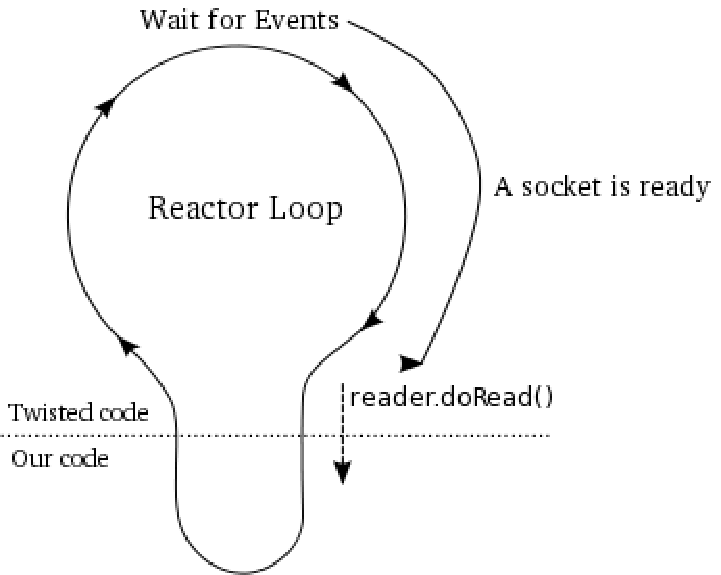
\includegraphics[width=0.5\textwidth]{images/reactor-doread.pdf}
    \caption{doRead callback\label{fig:reactor-doread}}
\end{center}
\end{figure}

Каждый раз, когда вызывается callback, 
из сокета считывается максимальное количество данных, после 
чего чтение прерывается без блокирования. Как было упомянуто в 
главе 3, Twisted не может предотвратить какие-то ни было 
проблемы в нашем коде, в том числе и блокирование. Чтобы это понять 
это, подправим наш код и посмотрим что получится. В той же 
директории, где находится Twisted клиент, расположен сломанный 
клиент в \href{http://github.com/jdavisp3/twisted-intro/blob/master/twisted-client-1/get-poetry-broken.py}{twisted-client-1/get-poetry-broken.py}. Этот клиент отличается следующим:

\begin{enumerate}
\item Сломанный клиент не заботится о том, чтобы установить socket в неблокирующий режим. 
\item callback doRead считываниет данные до закрытия сокета (то есть в этом случае 
происходит блокирование в момент, когда на сокете нет данных).
\end{enumerate}

Теперь попробуем запустить сломанный клиент:

\begin{scriptsize}\begin{verbatim}
python twisted-client-1/get-poetry-broken.py 10000 10001 10002
\end{verbatim}\end{scriptsize}

Получится примерно такой вывод:

\begin{scriptsize}\begin{verbatim}
Task 1: got 3003 bytes of poetry from 127.0.0.1:10000
Task 3: got 653 bytes of poetry from 127.0.0.1:10002
Task 2: got 623 bytes of poetry from 127.0.0.1:10001
Task 1: 3003 bytes of poetry
Task 2: 623 bytes of poetry
Task 3: 653 bytes of poetry
Got 3 poems in 0:00:10.132753
\end{verbatim}\end{scriptsize}


Несмотря на порядок задач, вывод похож на тот, что был 
у блокирующегося клиента. Это потому что наш сломанный 
клиент и является блокирующимся клиентом. Используя блокирующийся 
вызов recv в нашем callback'е, мы превратили нашу 
асинхронную Twisted программу в синхронную. 


Своего рода многозадачность, которую предоставляет 
event loop в Twisted, кооперативная. Twisted 
скажет нам, когда можно читать или писать в файловый 
дескриптор, но мы должны передавать данные без блокирования. 
И мы должны избегать блокирующих вызов, подобных os.system. 
Более того, если мы имеем длительную вычислительную 
задачу (потребляющую процессор), за нами разделить 
ее на несколько меньших кусков так, чтобы другие задачи  
могли выполнять ввод-вывод.


% Note that there is a sense in which our broken client still works: it does manage to download all the poetry we asked it to. It’s just that it can’t take advantage of the efficiencies of asynchronous I/O. Now you might notice the broken client still runs a lot faster than the original blocking client. That’s because the broken client connects to all the servers at the start of the program. Since the servers start sending data immediately, and since the OS will buffer some of the incoming data for us even if we don’t read it (up to a limit), our blocking client is effectively receiving data from the other servers even though it is only reading from one at a time.

Заметьте, что есть смысл в том, что наш сломанный клиент 
все еще работает: он скачивает запрашиваемую поэзию. 
Единственное, что он не использует преимущества асинхронного 
ввода-вывода. Можно заметить, что сломанный клиент работает 
намного быстрее, чем первоначальный блокирующийся клиент. 
Это потому что сломанный клиент соединяется со всеми 
серверами при старте программы. Поскольку сервера начинают отправлять 
данные немедленно, и поскольку операционная система буферизирует 
некоторые приходящие данные для нас (до какого-то фиксированного предела), 
даже если мы их не читали, наш блокирующий клиент 
эффективно получает данные из других серверов, даже если 
происходит поочереденое считывание.


%But this “trick” only works for small amounts of data, like our short poems. If we were downloading, say, the three 20 million-word epic sagas that chronicle one hacker’s attempt to win his true love by writing the world’s greatest Lisp interpreter, the operating system buffers would quickly fill up and our broken client would be scarcely more efficient than our original blocking one.


Но этот "трюк" работает только для небольшого объема данных, 
подобных нашим поэмам. Если бы мы скачивали, скажем, эпические 
саги с 20 милионнами слов, являющиеся записями одного 
хакера в попытке написать великолепный интерпретатор
\href{http://en.wikipedia.org/wiki/Lisp\_(programming\_language)}{Lisp}, 
буферы операционной системы быстро бы заполнились, и наш 
сломанный клиент был бы не эффективнее нашего первоначального 
блокирующего клиента.

\subsection{Резюме}

%I don’t have much more to say about our first Twisted poetry client. You might note the connectionLost callback shuts down the reactor after there are no more PoetrySockets waiting for poems. That’s not such a great technique since it assumes we aren’t doing anything else in the program other than download poetry, but it does illustrate a couple more low-level reactor APIs, removeReader and getReaders.


Больше нечего сказать о нашей первой Twisted версии клиента. 
Заметьте, что 
\href{http://github.com/jdavisp3/twisted-intro/blob/master/twisted-client-1/get-poetry.py#L74}{connectionLost} 
callback завершает reactor после того, как закончились все 
ожидающие поэм PoetrySocket'ы. Это не особо хороший способ, 
поскольку он предполагает, что в программе мы ничего кроме 
скачивания поэзии не делаем, но позволяет проиллюстрировать 
несколько низкоуровневых реакторных API: removeReader и getReaders.


%There are Writer equivalents to the Reader APIs we used in this client, and they work in analogous ways for file descriptors we want to monitor for sending data to. Consult the interfaces file for more details. The reason reading and writing have separate APIs is because the select call distinguishes between those two kinds of events (a file descriptor becoming available for reading or writing, respectively). It is, of course, possible to wait for both events on the same file descriptor.

Существуют Writer API, эквивалентные Reader API, которые 
мы использовали, и они работают также для файловых дескрипторов, 
которые мы хотим мониторить, чтобы отправить данные. Просмотрите  
\href{http://twistedmatrix.com/trac/browser/tags/releases/twisted-8.2.0/twisted/internet/interfaces.py}{interface'ы} 
для ознакомления с деталями. Причина, по которой чтение и запись 
имеют отдельные API, связана с тем, что вызов select 
отличает виды событий (файловый дескриптор доступен на 
чтение или запись). Конечно же, можно ожидать обоих событий 
на одном и том же файловом дескрипторе. 


%In Part 5, we will write a second version of our Twisted poetry client using some higher-level abstractions, and learn some more Twisted Interfaces and APIs along the way.

В следующей главе, мы напишем вторую версию нашего Twisted 
поэтического клиента, используя некоторые высокоуровневые 
абстракции, и по пути изучим несколько Twisted интерфейсов и 
API. 


\subsection{Упражнения}

\begin{enumerate}

%1. Fix the client so that a failure to connect to a server does not crash the program.
\item Исправьте клиент так, чтобы сбой при соединении с сервером не рушил программу.

%2. Use callLater to make the client timeout if a poem hasn’t finished after a given interval. Read about the return value of callLater so you can cancel the timeout if the poem finishes on time.
\item Воспользуйтесь callLater, для того, чтобы сделать клиентский 
timeout, в случае, если поэма не скачалась за заданный временной 
интервал. Прочитайте о возвращаемом значении callLater, для того, 
чтобы вы могли отменить таймер, в случае, если поэма скачалась 
во время.

\end{enumerate}
